
   \section{Lag Compensation}

   \begin{frame}
      \frametitle{Lag Compensation}
      \begin{center}
      \Huge{Lag Compensation}
      \end{center}
   \end{frame}
   
   \begin{frame}
      \frametitle{Lag Compensation}
      \begin{itemize}
         \item An in depth discussion of lag/latency compensation goes beyond
         the scope of this training.  Please see the following paper for more
         detailed information on the subject:
      \end{itemize}
         \begin{scriptsize}
         \begin{quote}
         \textit{R. Phillips, E. Crues, Time Management Issues and Approaches
         for Real Time HLA Based Simulations, Proceedings of the Fall 2005
         Simulation Interoperability Workshop and Conference, Fall 2005.}
         \end{quote}
         \end{scriptsize}
      \begin{itemize}
         \item Lag Compensation is an attempt to correct for the time difference
         between when a state is published at one federate and received at
         another federate.
         \item Using TrickHLA lag compensation consists of four steps:
         \begin{itemize}
            \item Step 1: Extend the \texttt{TrickHLALagCompensation} class and
            implement the \texttt{sending\_lag\_compensation()} and
            \texttt{receive\_lag\_compensation()} virtual functions.
            \item Step 2: In the \texttt{S\_define} file add a lag-compensation
            object to each simulation object that needs to perform lag compensation.
            \item Step 3: Configure lag compensation in the \texttt{input.py} file.
            \item Step 4: Update the object attributes in the \texttt{input.py}
            file to use the lag compensated Trick simulation variable.
         \end{itemize}
      \end{itemize}
   \end{frame}

   \begin{frame}[fragile]
      \frametitle{Lag Compensation}
      \framesubtitle{Step 1: Extend the \texttt{TrickHLALagCompensation} Class}
      \begin{itemize}
         \item Step 1: Extend the \texttt{TrickHLALagCompensation} class and
         implement the \texttt{sending\_lag\_compensation()} and
         \texttt{receive\_lag\_compensation()} virtual functions. Example in
         \texttt{SineLagCompensation.hh}:
      \vspace{0.2cm}
\begin{Verbatim}[frame=single, fontsize=\tiny]
#include "SineData.hh"
#include "TrickHLA/include/TrickHLALagCompensation.hh"

class SineLagCompensation : public TrickHLALagCompensation
{
...
public:
   // From the TrickHLALagCompensation class.
   virtual void sending_lag_compensation( double current_time, double dt );

   // From the TrickHLALagCompensation class.
   virtual void receive_lag_compensation( double current_time, double dt );
...
};
\end{Verbatim}
         \item TrickHLA will automatically call the send or receive lag
         compensation functions at the appropriate time.
      \end{itemize}
   \end{frame}

   \begin{frame}[fragile]
      \frametitle{Lag Compensation}
      \framesubtitle{Step 2: Add Lag-compensation Object to \texttt{S\_define}}
      \begin{itemize}
         \item Step 2: In the \texttt{S\_define} file add a lag-compensation
         object to each simulation object that needs to perform lag compensation.
         Make sure to initialize your lag-compensation object if it needs it.
      \end{itemize}
\begin{Verbatim}[frame=single, fontsize=\scriptsize]
   class ASimObject : public Trick::SimObject {
      ...
      SineData     sim_data;
      SineData     lag_comp_data;
      SinePacking            packing;
      SineLagCompensation    lag_compensation;
      SineInteractionHandler interaction_handler;

      ASimObject() {
        P50 ("initialization") packing.initialize( &sim_data );
        P50 ("initialization") lag_compensation.initialize( &sim_data, 
                                                            &lag_comp_data );
        ...
      }
   };
\end{Verbatim}
   \end{frame}

   \begin{frame}[fragile]
      \frametitle{Lag Compensation}
      \framesubtitle{Step 3: Configuration}
      \begin{itemize}
         \item Step 3: Configure lag compensation in the \texttt{input.py} file.
         \vspace{0.2cm}
\begin{Verbatim}[frame=single, fontsize=\scriptsize]
THLA.manager.objects[0].lag_comp      = A.lag_compensation
THLA.manager.objects[0].lag_comp_type = trick.THLA_LAG_COMP_SENDING
\end{Verbatim}
      \item The supported lag compensation types are:
         \begin{itemize}
            \item \texttt{THLA\_LAG\_COMP\_NONE}  (default)
            \item \texttt{THLA\_LAG\_COMP\_SENDING}
            \item \texttt{THLA\_LAG\_COMP\_RECEIVE}
         \end{itemize}
      \end{itemize}
   \end{frame}

   \begin{frame}[fragile]
      \frametitle{Lag Compensation}
      \framesubtitle{Step 4: Update Object Attributes}
      \begin{itemize}
         \item Step 4: Update the attribute \texttt{trick\_name} field in the
         \texttt{input.py} file to use the lag compensated Trick simulation variable.
         \item If the lag compensation type is \texttt{THLA\_LAG\_COMP\_NONE}:
         \vspace{0.2cm}
\begin{Verbatim}[frame=single, fontsize=\scriptsize]
THLA.manager.objects[0].attributes[1].FOM_name   = "Value"
THLA.manager.objects[0].attributes[1].trick_name = "A.sim_data.value"
\end{Verbatim}
      \item If the lag compensation type is \texttt{THLA\_LAG\_COMP\_SENDING}
      or \texttt{THLA\_LAG\_COMP\_RECEIVE}:
         \vspace{0.2cm}
\begin{Verbatim}[frame=single, fontsize=\scriptsize]
THLA.manager.objects[0].attributes[1].FOM_name   = "Value"
THLA.manager.objects[0].attributes[1].trick_name = "A.lag_comp_data.value"
\end{Verbatim}
      \end{itemize}
   \end{frame}

   \begin{frame}
      \frametitle{Lag Compensation}
      \framesubtitle{Combinations}
      \begin{itemize}
         \item The five logical combinations of lag compensation between two
         federates is shown in the table below:
      \end{itemize}
\begin{tiny}
\begin{center}
\begin{tabular}{|l|l|l|} \hline
\textbf{Lag Comp. Type} & \textbf{A-side-Federate} & \textbf{P-side-Federate} \\ \hline
None & Publish: THLA\_LAG\_COMP\_NONE   & Subscribe: THLA\_LAG\_COMP\_NONE \\
     & Subscribe: THLA\_LAG\_COMP\_NONE & Publish: THLA\_LAG\_COMP\_NONE \\ \hline
Sending-side & Publish: THLA\_LAG\_COMP\_SENDING & Subscribe: THLA\_LAG\_COMP\_NONE \\
             & Publish: THLA\_LAG\_COMP\_SENDING & Subscribe: THLA\_LAG\_COMP\_NONE \\ \hline
Receive-side & Publish: THLA\_LAG\_COMP\_NONE & Subscribe: THLA\_LAG\_COMP\_RECEIVE \\
             & Publish: THLA\_LAG\_COMP\_NONE & Subscribe: THLA\_LAG\_COMP\_RECEIVE \\ \hline
Sending- and & Publish: THLA\_LAG\_COMP\_SENDING & Subscribe: THLA\_LAG\_COMP\_RECEIVE \\
Receive-side & Subscribe: THLA\_LAG\_COMP\_NONE  & Publish: THLA\_LAG\_COMP\_NONE \\ \hline
Sending- and & Publish: THLA\_LAG\_COMP\_NONE    & Subscribe: THLA\_LAG\_COMP\_NONE \\
Receive-side & Publish: THLA\_LAG\_COMP\_SENDING & Subscribe: THLA\_LAG\_COMP\_RECEIVE \\ \hline
\end{tabular}
\end{center}
\end{tiny}
      \begin{itemize}
         \item "Publish" refers to the attributes the federate is configured to
         send data for.
         \item "Subscribe" refers to the attributes the federate is configured
         to receive data for.
      \end{itemize}
   \end{frame}

   \begin{frame}
      \frametitle{Lag Compensation}
      \framesubtitle{TrickHLA jobs in THLA.sm}
      \begin{figure}
      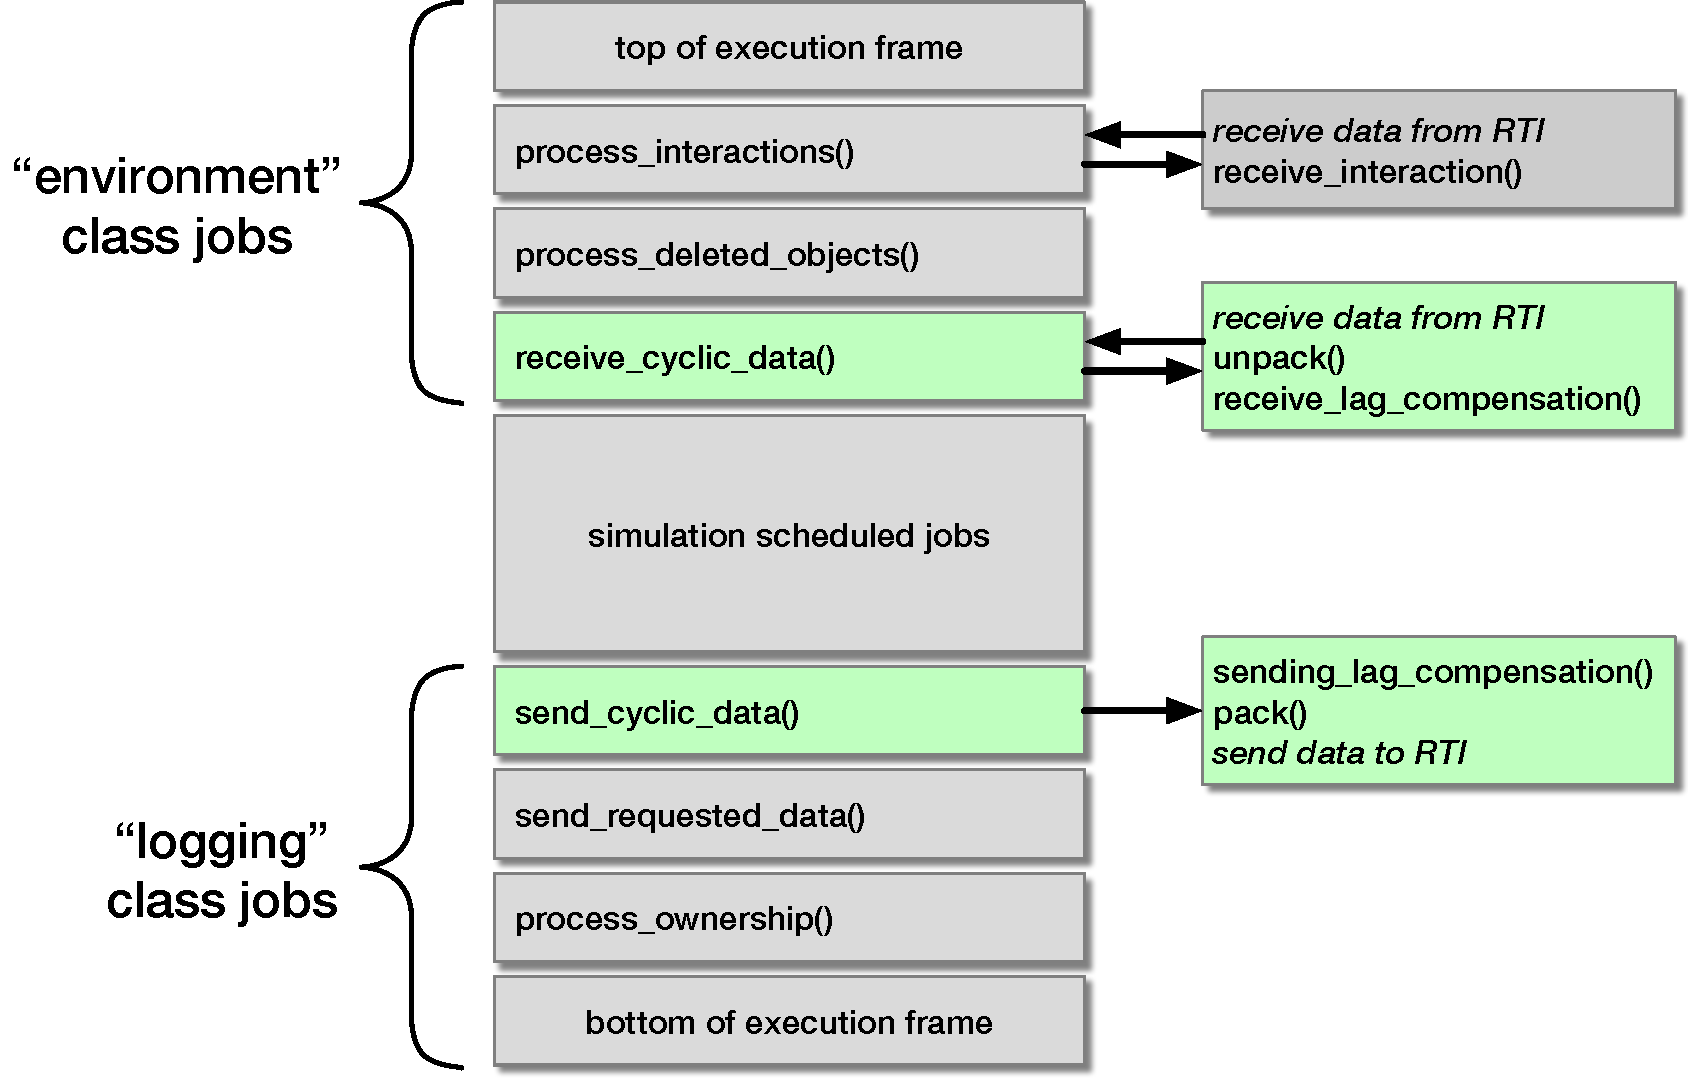
\includegraphics[scale=0.4]{TutorialTHLALagCompJobs.pdf}
      \end{figure}
   \end{frame}

